\title{Informe de Estadística en Física Experimental: Ejercicio 13 de la guia 8,  13 y 14 de la  Guía 9}
\author{Andrés Babino}

\begin{document}
\maketitle
\section{Introducción}
El lenguaje utilizado para programar todas los ítems fue Python.
El código utilizado para generar los datos, gráficos y este mismo informe fue controlado con git, tiene licencia MIT y está almacenado en \url{https://github.com/ababino/efe}.

\section*{Guía 8}
\subsection*{Ejercicio 13}
\subsubsection*{Ítem a}
Como las mediciones son a tiempo fijo la variable aleatoria es poissoniana.
Si se desea ajustar la curva $y(t) = a_1 + a_2 e^{-t/209.69s} + a_3 e^{-t/34.244s}$ a un conjunto de datos se deben usar las fórmulas de cuadrados mínimos lineal.
Los parámetros quedan determinados por:
$$
\vec{\theta} = {(AV^{-1}A)}^{-1}AV^{-1}y
$$
Donde $\theta$ es el vector de parámetros $(a_1, a_2, a_3)$ y $A$ es una matriz que tiene unos en la primera columna, $e^{-t_i/209.69s}$, en la segunda y $e^{-t_i/34.244s}$ en la tercera.
$V$ es la matriz de covarianza de la variable independiente.
En este caso la matriz es diagonal porque los datos no están correlacionados y la varianza es poisson.

La matriz de covarianza de los parámetros ajustados se puede calcular de la siguiente manera:
$$
Cov(\vec{\theta}) = {(AV^{-1}A)}^{-1}
$$
Los resultados de este ajuste fueron:
$$
\vec{\theta} = (10.1, 128, 960)
$$
$$
V(\vec{\theta}) =\left(
\begin{matrix}
0.70 &-3.3 & 7.0 \\
-3.3 & 38 &-99 \\
7.0  & -99 & 1000
\end{matrix} \right)
$$

Usando estos datos podemos calcular el valor esperado del cociente $a_2/a_3$ y usando la fórmula de propagación de errores su error:

$$
\frac{a_2}{a_3} = 0.1339 \pm 0.0095
$$

\subsubsection*{Ítem b}
Si $a_4$ y $a_5$ son desconocidos la función a ajustar no es lineal en los parámetros.
Minimizando la función $\chi^2$ con respecto a los parámetros obtenemos:
$$
\vec{\theta}=(10\ 128\ 957\  210\  34)
$$
$$
Cov(\vec{\theta}) = \left(
\begin{matrix}
4.0  & 34   &  0.44 & -61  & -3.1\\
34   & 530  & 150   & -74  & -53\\
0.44 & 150  & 2600  & -98  & -79\\
-61  & -740 & -98   & 1200 & 69\\
-3.1 & -53  & -79   & 69.  & 7.5
\end{matrix}
\right)
$$
\subsubsection*{Ítem c}
En este caso la función $\chi^2$ es:
$$
t(a_1, a_2, a_3, a_4, a_5) = \sum_{i=1}^N \frac{{\left(y_i-a_1 - a_2 e^{-t/a_4} - a_3 e^{-t/a_5}\right)}^2}{y_i}
$$
que debido a que los parámetros $a_4$ y $a_5$ están en las exponenciales el $\chi^2$ no es cuadrático en los parámetros.

Si en el argumento de $t$ dejamos fijo $a_1=a_1^*$, $a_2=a_2^*$ y $a_3=a_3^*$, los valores óptimos ya calculados, obtenemos una función de $a_4$ y $a_5$.
Otra opción es para cada par $(a_4, a_5)$ calcular la terna óptima $(a_1, a_2, a_3)$ y con ellos calcular el $\chi^2$.
En el gráfico de la figura\ref{fig:fig1} se muestra la curva de nivel $t=t_{\min} + 1$ para las dos funciones.

\begin{figure}
\centering
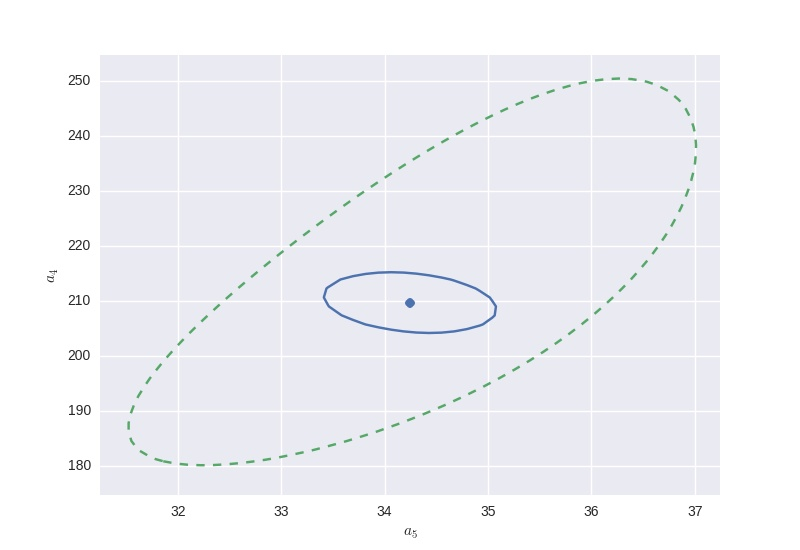
\includegraphics[width=0.75\textwidth]{fig1.jpg}
\caption[]{}
\label{fig:fig1}
\end{figure}


El conjunto de los $\vec \theta$ para los cuales la función $\chi^2=\delta$ es un conjunto de nivel (el equivalente multidimensional de las curvas de nivel).
Este conjunto es una hipersuperficie de $4$ dimensiones que lógicamente no se puede visualizar.
Si esta hipersuperficie correspondiese a una función cuadrática en los parámetros (con matriz de covarianza definida positiva) al alejarnos del hipervéritce (el valor óptimo) de esta hiperparábola el valor de la función aumentaría siempre.
Sin embargo, este no es el caso, por lo tanto cuando nos alejamos del valor óptimo no siempre el valor de $\chi^2$ aumenta.

En conclusión las dos curvas son diferentes cortes del la hipersuperficie de nivel.
La curva azul corresponde al corte en el plano  $(\theta_1, \theta_2, \theta_3)=(\theta_1^*, \theta_2^*, \theta_3^*)$ y a los límites de $(\theta_1, \theta_2)$ corresponden a los límites que tendrían si $\chi^2$ fuese cuadrático en los parámetros.
Como no los es, existen puntos del espacio $(\theta_1, \theta_2)$ más alejados aún del centro que tienen valores de $\chi^2$ menores a nuestro umbral $\delta$.
Estos puntos tienen otros valores de $(\theta_1, \theta_2, \theta_3)$ pero pertenecen a la hipersuperficie de nivel (o están dentro de ella).

\subsubsection*{Ítem d}
Para calcular los intervalos de $68\%$ de nivel de confianza para cada variable por separado habría que integrar la distribución conjunta en todas las otras variables y calcular la región de área $0.68$
Como no conocemos la distribución exacta lo que podemos hacer es aproximarla por una $\chi^2_1$ que cerca de los parámetros óptimos debe ser una buena aproximación.
En este caso el intervalo del $68\%$ está comprendido a más menos un $\sigma$ del valor óptimo, es decir:

$$
\theta_4 \in (175, 245)\ 68\%\ c.l.
$$
$$
\theta_5 \in (31.3, 36.7) \ 68\%\ c.l.
$$

\subsubsection*{Ítem e}
En el caso de que se quiera calcular el intervalo de $95\%$ habría que apartarse $2\sigma$ del valor óptimo, pero esta aproximación sería menos exacta aún.

Si lo que queremos es el contorno conjunto ahora podemos aproximar la probabilidad conjunta como una binormal y por lo tanto la variable  $Q = (\theta_4-\theta_4^*, \theta_5-\theta_5^*) V(\theta_4, \theta_5)^{-1} (\theta_4-\theta_4^*, \theta_5-\theta_5^*)^t$ debe seguir una distribución $\chi^2_2(Q)$.
De este modo encontramos una elipse definida por $Q(\theta_4, \theta_5)=5.99$ que es el valor para el cual $\int_0^{5.99}\chi^2_2(x)dx=0.95$.

\section*{Guía 9}
\subsection*{Ejercicio 13}
\subsubsection*{Ítem a}
Por simple inspección ocular se pueden ordenar los histogramas como se muestra en la figura\ref{fig:hists}
\begin{figure}
\centering
\begin{subfigure}[b]{0.3\textwidth}
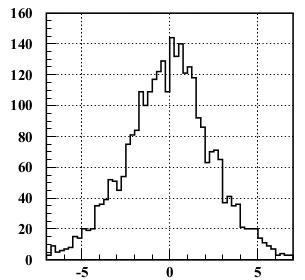
\includegraphics[width=0.84\textwidth]{hist3.jpg}
\end{subfigure}
\begin{subfigure}[b]{0.3\textwidth}
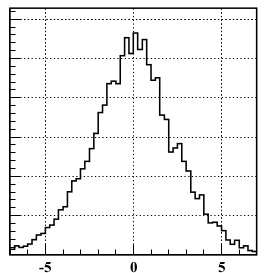
\includegraphics[width=0.75\textwidth]{hist2.jpg}
\end{subfigure}
\begin{subfigure}[b]{0.3\textwidth}
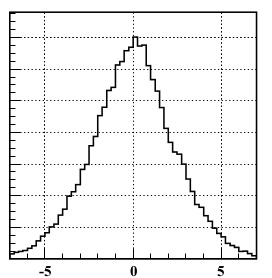
\includegraphics[width=0.75\textwidth]{hist1.jpg}
\end{subfigure}
\caption[]{}
\label{fig:hists}
\end{figure}

\subsubsection*{Ítem b}
En la figura\ref{fig:fig2} se muestra un histograma de los primeros $3000$ datos.
Sobre estos se graficó las cuentas esperadas asumiendo una distribución $N(0, 2.5)$.
Si aplicamos un test $\chi^2$ sobre estos datos obtenemos que un valor $\chi^2=67$.
El número de grados de libertad de la $\chi^2$ es $56$ (el número de bines) por lo tanto el p valor del test es $p-val=0.15$.
Con este p valor no podemos rechazar la hipótesis nula.

\begin{figure}
\centering
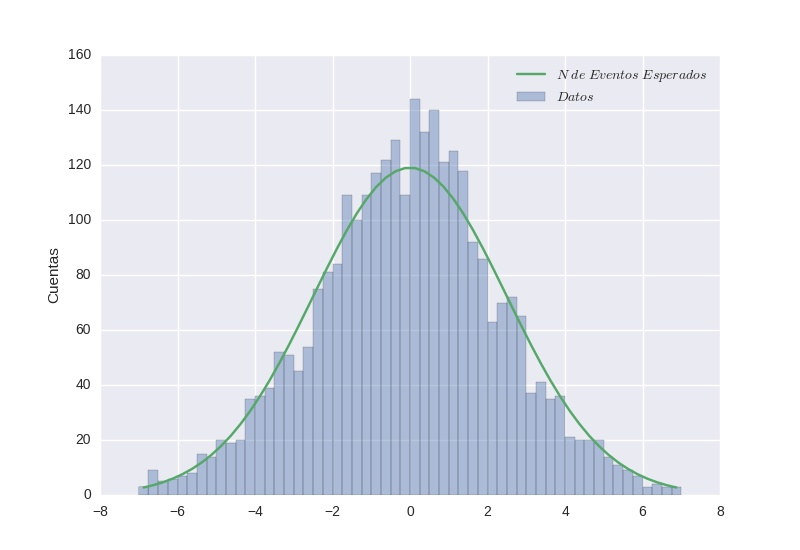
\includegraphics[width=0.75\textwidth]{fig2.jpg}
\caption[]{}
\label{fig:fig2}
\end{figure}

Si sobre los mismos datos aplicamos los tests de Kolmolgorov y de Cramer Von-Mises obtenemos valores $t_k=0.032$ y $t_c=0.0015$ respectivamente.
Comparando con las tablas de valores críticos vemos que en los dos casos podemos rechazar la hipótesis nula con un $99\%$ de nivel de confianza.

\subsubsection*{Ítem c}
En los gráficos de la figura\ref{fig:fig3} se muestra la variación de los estadísticos y sus valores críticos para distinto tamaños de muestra.
Se puede observar que a medida que el tamaño de la muestra crece todos los test rechazan la hipótesis nula con más de $99\%$ de nivel de confianza.

\begin{figure}
\centering
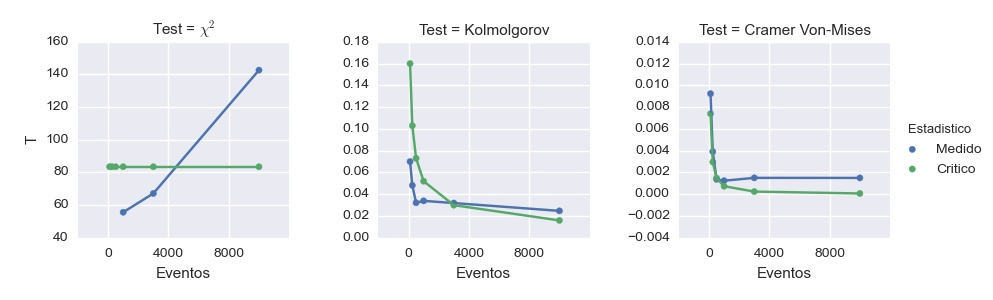
\includegraphics[width=\textwidth]{fig3.jpg}
\caption[]{En azul se muestra el valor medidio de los estadísticos para distintos números de datos. En rojo se muestra el valor crítico de esos estádisticos para una significancia del $1\%$}
\label{fig:fig3}
\end{figure}


\subsection*{Ejercicio 14}
\subsubsection*{Ítem a}
Para 1000 realizaciones de los datos del ejercicio 7 de la guía 5 calculamos el $\chi^2$ correspondiente y los graficamos en un histograma en la figura \ref{fig:fig4}.
Sobre este histograma graficamos la distribución $\chi^2_{11}$ porque el número de datos es $11$ y observamos que se ajusta razonablemente bien.

\begin{figure}
\centering
\includegraphics[width=0.75\textwidth]{fig4.jpg}
\caption[]{}
\label{fig:fig4}
\end{figure}


Repetimos el mismo proceso, pero esta vez ajustando una curva para cada realización y calculando el $\chi^2$ correspondiente.
Como ahora estamos ajustando $2$ parámetros los valores de $\chi^2$ deben seguir una distribución de $9$ grados de libertad.
En el gráfico de la figura \ref{fig:fig5} se observa como ahora la distribución $\chi^2_9$ se ajusta mejor a los datos que la distribución $\chi^2_{11}$.

\begin{figure}
\centering
\includegraphics[width=0.75\textwidth]{fig5.jpg}
\caption[]{}
\label{fig:fig5}
\end{figure}

\end{document}
